\chapter{导言}

\section{经济学十大原理}

\subsection*{人们面临权衡取舍}

最常见的取舍在于对资源的分配, 另一种取舍在于如何平衡效率(社会能从稀缺资源中得到最大利益)与平等(经济成果在社会成员中平均分配). 

\subsection*{机会成本原理}

机会成本, 即为了得到某种东西而必须放弃的东西. 用粗糙的数学视角来看, 就是说在选择$A_1,\cdots ,A_n$之间存在一个关联$f$, 使得$f(A_1,\cdots ,A_n)$为定值$0$. 

\begin{example}{生产可能性边界}
	考虑一个电脑-汽车生产的模型. 在这个模型中, 让生产电脑的工人转而生产汽车, 将会导致汽车产量增加和电脑产量下降, 反之亦然. 因此, 我们可以用电脑产量作为机会成本来描述汽车产量. 
	\begin{figure}[H]
		\centering
		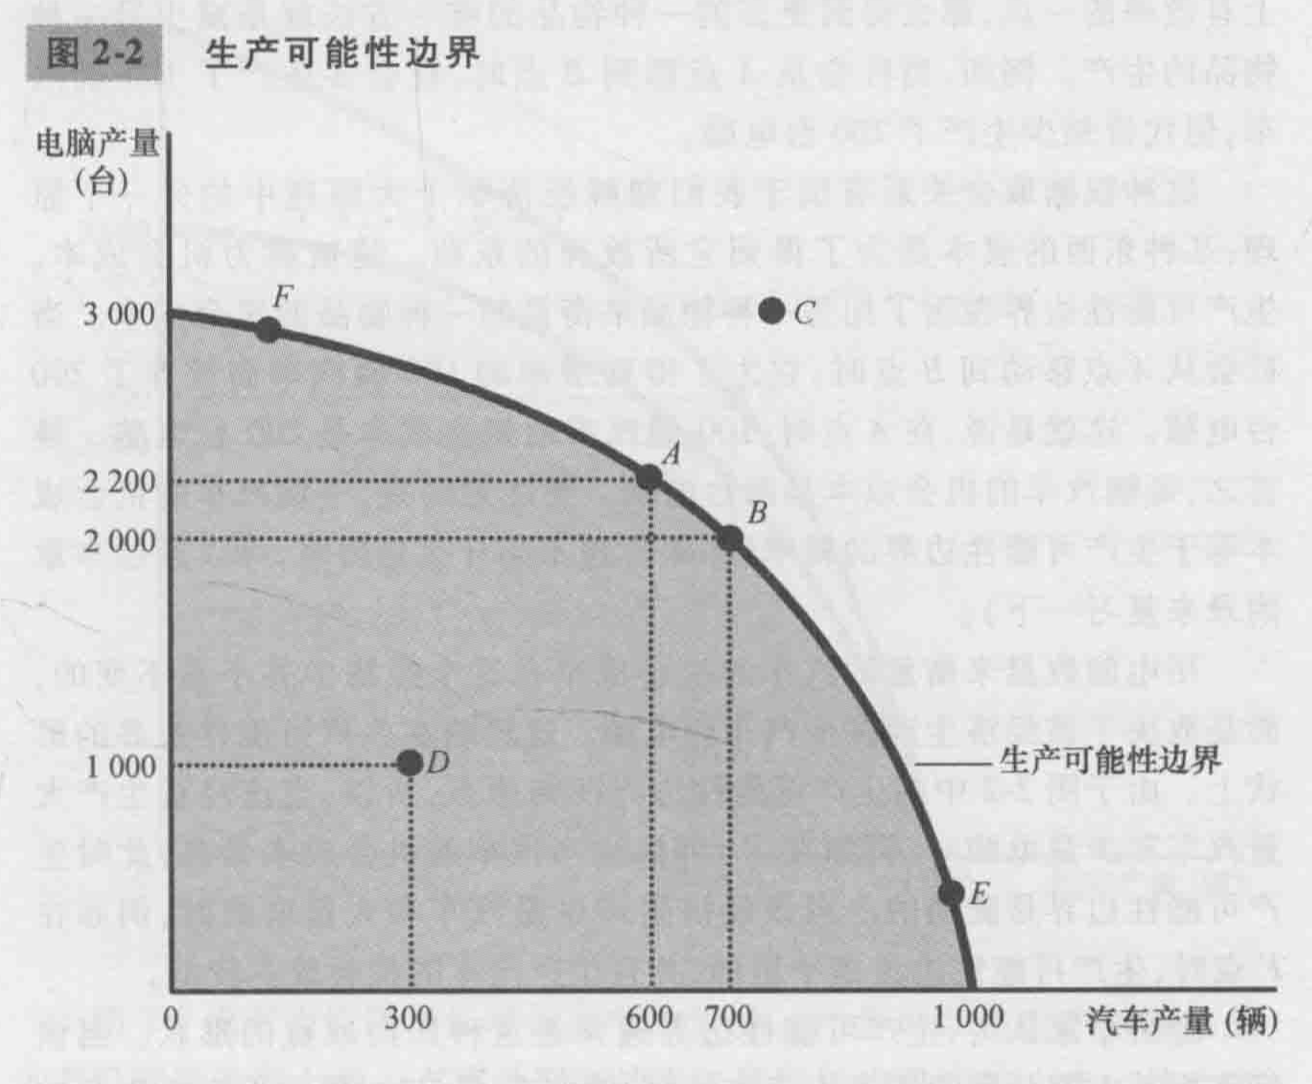
\includegraphics[width=8cm]{attachment/Fig2_2.png}
	\end{figure}
	从数学的视角来看, 两种产量$A_1,A_2$具有类似$A_1+A_2=C$的关系. 特别地, 极端追求汽车产量会让大量熟练于电脑生产的工人转而生产汽车, 这时付出很多电脑工人也只能推动汽车产量的微小变化, 因此越靠近$E$点, 一单位汽车所对应的电脑成本越高. 即是说整个曲线呈现上凸的形状. 
\end{example}

\subsection*{理性人考虑边际量}

实际上, 这个原理基于某种公设, 即所谓理性人(经济人)假设: \textit{人们总是以理性和利己的行为追求目标利益最大化}. 

用数学的话, 考虑一个将行为变成结果的函数$f$. 为了让$f(x)$取得最大值$M$, 可以先找到那些使得$f(x)$与$M$差距不大的$x$, 再在这些$x$(边际量)中找到$f(x)=M$的点. 

\begin{example}{沉没成本}
	已经付出且不可收回的成本, 就成为沉没成本. 按照边际分析的原理, 理性人不应当考虑沉没成本, 因为此时再付出多少都与沉没成本无关. (当然这是在不考虑个人情绪价值等的情况下)
\end{example}

\subsection*{人们会对激励做出反应}

在分析经济行为的后果时, 不仅要考虑其本身直接后果, 还要考虑其作为激励的影响. 

\begin{example}{关于弹性的直观认知}
	提高价格的确能增加生产者的单件收入, 但这会导致消费者的购买量减少, 总收益不一定增加. 注:实际上当需求弹性较小时收益会增加. 
\end{example}

\subsection*{比较优势原理: 贸易可以使每个人的状况都变得更好}

当贸易的两者各具有一方面的特长时, 贸易的优势是显然的. 实际上, 当其中一者具有绝对性优势时, 贸易也会带来改善. 





因此, 贸易可以让每个人都从事自己最擅长的活动. 















